%
% auth: Mattijs Korpershoek
% mail: <mattijs.korpershoek@gmail.com>
%

% {{{1 intro
\section{Technical contributions}
\subsection{Directions}
\begin{FrameWithSubSection}
    \begin{itemize}
        \item Customer features
        \item Open-sourcing a core component
    \end{itemize}
\end{FrameWithSubSection}


% {{{1 Customer features
\subsection{Features for customers}
\begin{FrameWithSubSection}
    \begin{itemize}
        \item More than \emph{80} patches delivered
        \item Code integrated into Intel's code base
        \item Software quality compliant
    \end{itemize}
\end{FrameWithSubSection}

% {{{2 xml validation
\subsubsection{Xml Validation at build time}
\begin{frame}
    \frametitle{XML Validation at build time}
    \begin{minipage}{0.4\textwidth}
        \begin{itemize}
            \item More than 40 000 lines of XML
            \item More than 500 errors within those files
            \item Automatic validation with XSD at build time
            \item Prevents from submitting erroneous data
        \end{itemize}
    \end{minipage}
    \begin{minipage}{0.5\textwidth}
        \flushright
        \includegraphics[height=0.85\textheight]{../../report/src/img/build-generation-after.pdf}
    \end{minipage}
\end{frame}

% {{{2 fixed point
\subsubsection{Fixed point parameter improvements}
\begin{frame}
    \frametitle{Fixed point parameter improvements}
    \begin{minipage}{0.5\textwidth}
        \begin{block}{Fixed point numbers}
            \begin{itemize}
                \item $Qn.m$ notation
                    \begin{itemize}
                        \item $n$ : fractional part
                        \item $m$ : integral part
                    \end{itemize}
                \item Rounding issues with conversion to floating point
                \item \lstinline{std::setPrecision()}
            \end{itemize}
        \end{block}
    \end{minipage}
    \begin{minipage}{0.4\textwidth}
        \flushright
        \begin{block}{Solution}
            \begin{itemize}
                \item Simple and elegant solution
                \item Behavior test suite
                \item Used in multiple Intel products
            \end{itemize}
        \end{block}
    \end{minipage}
    \begin{minipage}{\textwidth}
        \flushright
        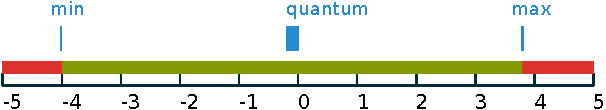
\includegraphics[width=\textwidth]{../../report/src/img/fixedPoint.pdf}
    \end{minipage}
\end{frame}

% {{{2 multimodem

\subsubsection{Multi modem support}
\begin{frame}
    \frametitle{Modem instance awareness}
    \begin{itemize}
        \item Voice processing algorithms
        \item Multiple modems for several phone carriers
        \item Big team effort of more than 200 patches
        \item Parameter-framework modem plugin
    \end{itemize}
\end{frame}

% {{{1 Opensourcing
\subsection{Open-sourcing the Parameter-framework}
\subsubsection{Context}
\begin{FrameWithSubSection}
    \begin{block}{Why open-sourcing this component?}
        \begin{itemize}
            \item Core component of Intel audio HAL
            \item Potential to become middleware standard
            \item Visibility
        \end{itemize}
    \end{block}
\end{FrameWithSubSection}

\subsubsection{Documentation}
\begin{frame}
    \frametitle{Newcomer documentation}
    \centering
    \begin{block}{Is the component ready for open-sourcing?}
        \begin{itemize}
            \item Code review and study
            \item Documentation for external contributors
            \item More than 450 lines of documentation
        \end{itemize}
    \end{block}
\end{frame}

\begin{frame}
    \frametitle{Newcomer documentation illustration}
    \centering
    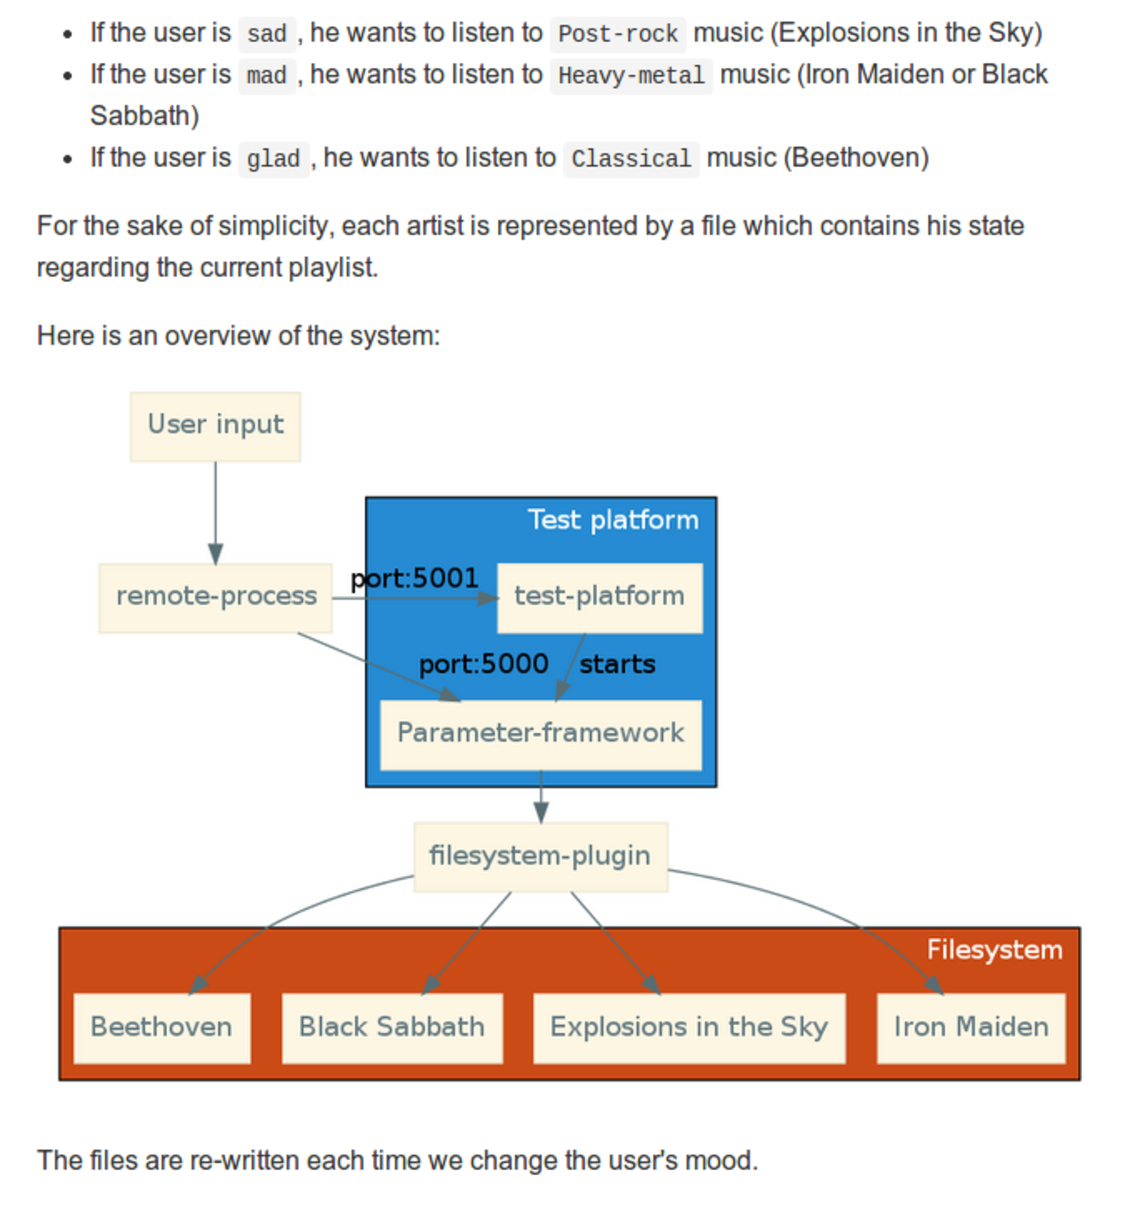
\includegraphics[height=0.85\textheight]{../../report/src/img/tutos.pdf}
\end{frame}

\subsubsection{Branch sync process}
\begin{frame}
    \frametitle{Branch sync process}
    \begin{block}{How to open-source the component?}
        \begin{itemize}
            \item Ensure external contributions are of quality
            \item Avoid maintenance of 2 divergent code bases
            \item Ensure no confidential information is exposed
        \end{itemize}
    \end{block}
\end{frame}

\begin{frame}
    \frametitle{Branch sync process}
    \centering
    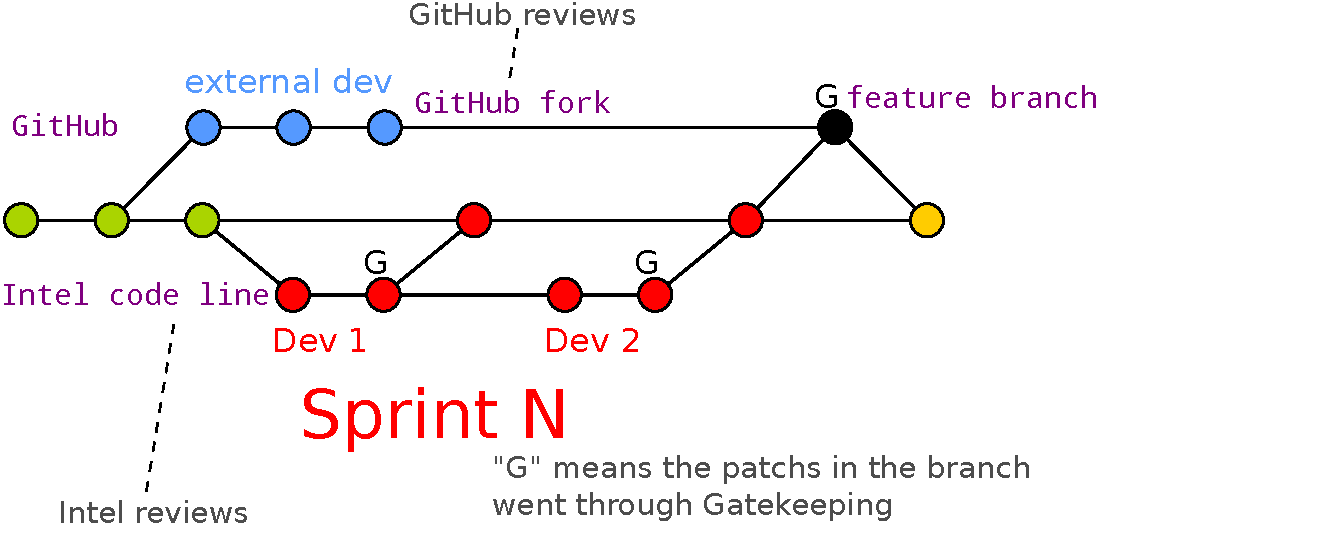
\includegraphics[width=\textwidth]{../../report/src/img/branches-process.pdf}
\end{frame}

\subsubsection{Open-sources projects}
\begin{frame}
    \frametitle{Projects which are open-source}
    \begin{block}{01org}
        \begin{itemize}
            \item \href{https://01.org/}{Intel Open Source Technology Center}
            \item \href{https://github.com/orgs/01org/teams/01-org-parameter-framework-owners}{GitHub organisation}
        \end{itemize}
   \end{block}
    \begin{block}{Projects on GitHub}
        \begin{itemize}
            \item Parameter-framework \href{https://github.com/01org/parameter-framework}{core}
            \item Parameter-framework \href{https://github.com/01org/parameter-framework-plugins-alsa}{ALSA plugin}
            \item Parameter-framework \href{https://github.com/01org/parameter-framework-plugins-filesystem}{filesystem plugin}
            \item Parameter-framework \href{https://github.com/01org/parameter-framework/wiki}{wiki}
            \item Parameter-framework \href{https://github.com/01org/parameter-framework-samples}{sample files}
        \end{itemize}
    \end{block}
\end{frame}

\begin{frame}
    \frametitle{GitHub top contributors}
    \centering
    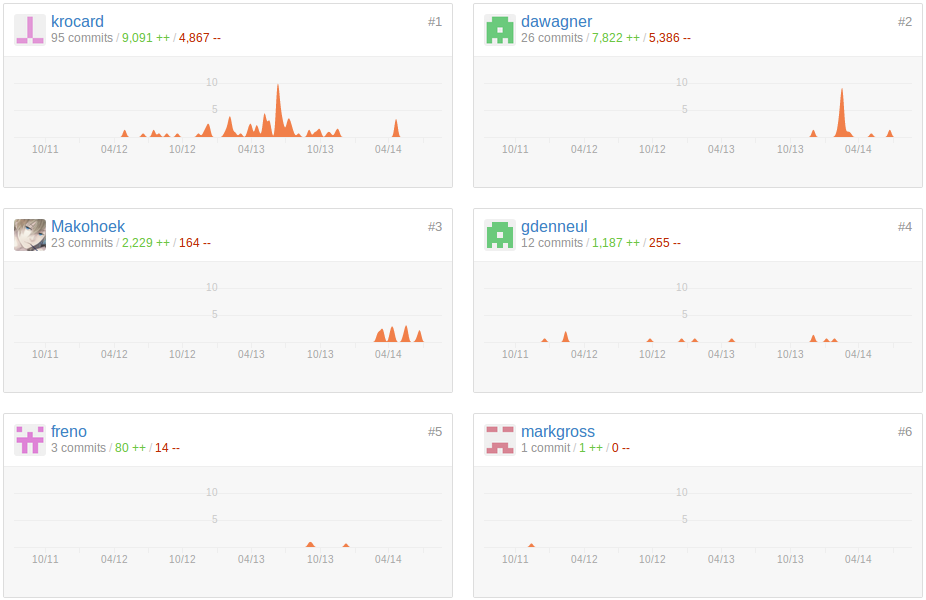
\includegraphics[width=\textwidth]{../../report/src/img/statsGitHub.png}
\end{frame}

